\documentclass[border=0pt]{standalone}
\usepackage{tikz}
\renewcommand{\familydefault}{\sfdefault}

\definecolor{bgtop}{HTML}{17134A}
\definecolor{bgbot}{HTML}{07061C}
\definecolor{steel}{HTML}{B4BFD6}
\definecolor{glass}{HTML}{0B0B2A}
\definecolor{gridc}{HTML}{2A2D63}
\definecolor{maskc}{HTML}{FF4D5E}
\definecolor{psd}{HTML}{4FD1FF}
\definecolor{base}{HTML}{F59E0B}

% plot area: x in [1.1, 10.9], y in [1.2, 7.0]; band edges at x = 4.19 and 7.81
\begin{document}
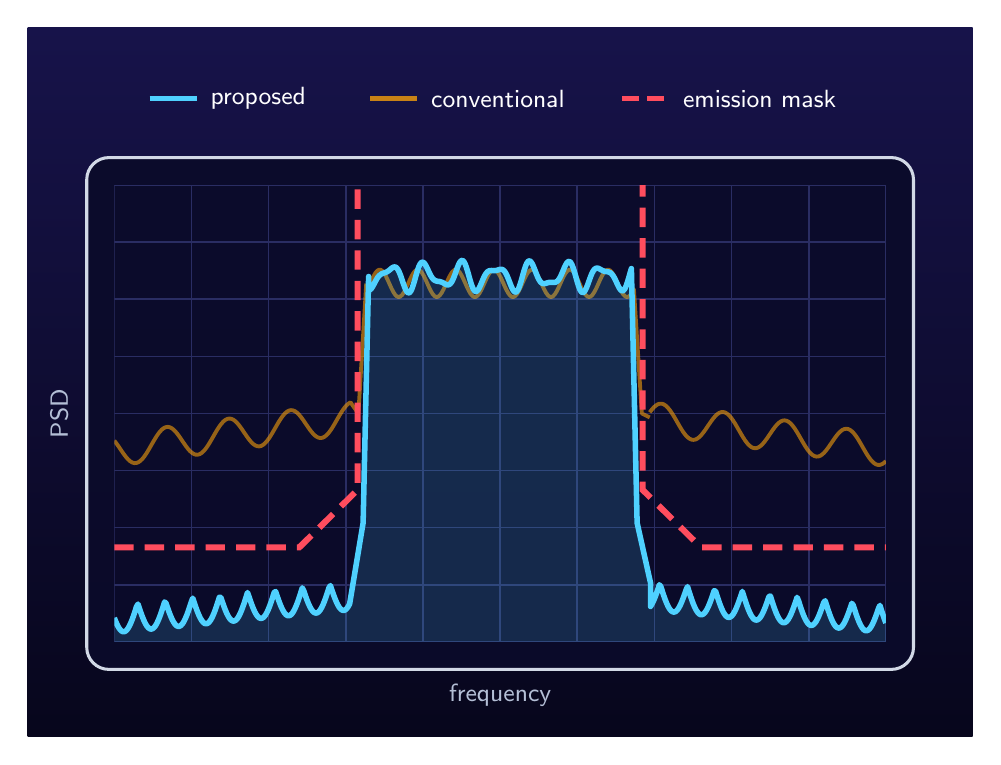
\begin{tikzpicture}
  \useasboundingbox (0,0) rectangle (12,9);
  \clip (0,0) rectangle (12,9);
  \shade[top color=bgtop,bottom color=bgbot] (0,0) rectangle (12,9);

  % analyzer panel
  \fill[glass,opacity=0.92,rounded corners=8pt] (0.75,0.85) rectangle (11.25,7.35);
  \draw[steel!60,line width=1.1pt,rounded corners=8pt] (0.75,0.85) rectangle (11.25,7.35);

  \begin{scope}
    \clip (1.10,1.20) rectangle (10.90,7.00);
    \foreach \i in {0,...,10}{\draw[gridc,line width=0.6pt] ({1.10+0.98*\i},1.20) -- ({1.10+0.98*\i},7.00);}
    \foreach \j in {0,...,8}{\draw[gridc,line width=0.6pt] (1.10,{1.20+0.725*\j}) -- (10.90,{1.20+0.725*\j});}

    % conventional precoder: out-of-band sidelobes break through the mask
    \draw[base,opacity=0.6,line width=1.4pt,line join=round]
      plot[domain=1.10:4.10,samples=120] (\x,{1.2+5.8*(0.49+0.035*sin(deg(\x*8))-0.07*(4.10-\x)/3.0)})
      -- (4.20,4.10) -- (4.30,5.75)
      plot[domain=4.30:7.70,samples=150] (\x,{1.2+5.8*(0.785+0.03*sin(deg(\x*13)))})
      -- (7.80,4.10) -- (7.90,4.05)
      plot[domain=7.90:10.90,samples=120] (\x,{1.2+5.8*(0.49+0.035*sin(deg(\x*8))-0.07*(\x-7.90)/3.0)});

    % proposed: in-band plateau, steep skirts, out-of-band held under the mask
    \fill[psd,opacity=0.16]
      (1.10,1.20)
      -- plot[domain=1.10:4.09,samples=160] (\x,{1.2+5.8*(0.13-0.06*abs(sin(deg(\x*9)))-0.05*(4.09-\x)/2.99)})
      -- (4.26,2.71) -- (4.33,5.84)
      -- plot[domain=4.33:7.67,samples=200] (\x,{1.2+5.8*(0.80+0.025*sin(deg(\x*14))+0.012*sin(deg(\x*23)))})
      -- (7.74,2.71) -- (7.91,1.95)
      -- plot[domain=7.91:10.90,samples=160] (\x,{1.2+5.8*(0.13-0.06*abs(sin(deg(\x*9)))-0.05*(\x-7.91)/2.99)})
      -- (10.90,1.20) -- cycle;
    \draw[psd,line width=2.0pt,line join=round]
      plot[domain=1.10:4.09,samples=160] (\x,{1.2+5.8*(0.13-0.06*abs(sin(deg(\x*9)))-0.05*(4.09-\x)/2.99)})
      -- (4.26,2.71) -- (4.33,5.84)
      -- plot[domain=4.33:7.67,samples=200] (\x,{1.2+5.8*(0.80+0.025*sin(deg(\x*14))+0.012*sin(deg(\x*23)))})
      -- (7.74,2.71) -- (7.91,1.95)
      -- plot[domain=7.91:10.90,samples=160] (\x,{1.2+5.8*(0.13-0.06*abs(sin(deg(\x*9)))-0.05*(\x-7.91)/2.99)});

    % spectral emission mask
    \draw[maskc,line width=2.2pt,dash pattern=on 7pt off 4pt]
      (1.10,2.40) -- (3.45,2.40) -- (4.19,3.13) -- (4.19,7.10);
    \draw[maskc,line width=2.2pt,dash pattern=on 7pt off 4pt]
      (7.81,7.10) -- (7.81,3.13) -- (8.55,2.40) -- (10.90,2.40);
  \end{scope}

  % axis hints
  \node[font=\small,text=steel] at (6.0,0.52) {frequency};
  \node[font=\small,text=steel,rotate=90] at (0.40,4.10) {PSD};

  % legend
  \begin{scope}[font=\small,text=white!88]
    \draw[psd,line width=2.0pt] (1.55,8.10) -- (2.15,8.10); \node[anchor=west] at (2.20,8.10) {proposed};
    \draw[base,opacity=0.8,line width=1.6pt] (4.35,8.10) -- (4.95,8.10); \node[anchor=west] at (5.00,8.10) {conventional};
    \draw[maskc,line width=2.0pt,dash pattern=on 6pt off 3pt] (7.55,8.10) -- (8.15,8.10); \node[anchor=west] at (8.20,8.10) {emission mask};
  \end{scope}
\end{tikzpicture}
\end{document}
